% Search for all the places that say "PUT SOMETHING HERE".

\documentclass[11pt]{article}
\usepackage{amsmath,textcomp,amssymb,geometry,graphicx,enumerate}
\usepackage{float}
\def\Name{Yide Shentu}  % Your name
\def\SID{25745510}  % Your student ID number
\def\Homework{2} % Number of Homework
\def\Session{Fall 2016}


\title{CS189--Fall 2016 --- Homework \Homework\ Solutions}
\author{\Name, SID \SID}
\markboth{CS189--\Session\  Homework \Homework\ \Name}{CS189--\Session\ Homework \Homework\ \Name}
\pagestyle{myheadings}
\date{}

\newenvironment{qparts}{\begin{enumerate}[{(}a{)}]}{\end{enumerate}}
\def\endproofmark{$\Box$}
\newenvironment{proof}{\par{\bf Proof}:}{\endproofmark\smallskip}

\textheight=9in
\textwidth=6.5in
\topmargin=-.75in
\oddsidemargin=0.25in
\evensidemargin=0.25in
%\setboolean{@twoside}{false}
\usepackage{pdfpages}
\begin{document}
\maketitle


\section*{1. Visualizing Eigenvectors of Gaussian Covariance Matrix}
\begin{figure}[H]
\begin{center}
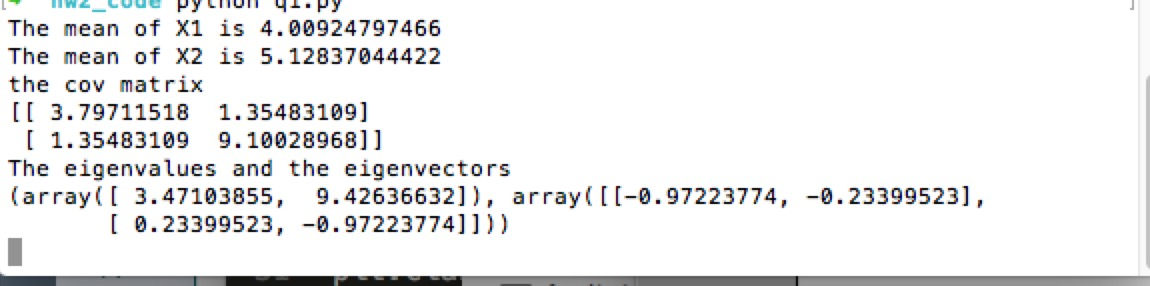
\includegraphics[scale=0.3]{q1}
\caption{Output of problem1}
\end{center}
\end{figure}
\subsection*{a)}
From figure 1, mean of X1 is 4.01 and mean of X2 is 5.13
\subsection*{b)}
From figure 1, 
\begin{center}
  \begin{tabular}{ | c c | }
 
    3.80 & 1.35 \\ 
    1.35 & 9.1 \\ 

  \end{tabular}
\end{center}
\subsection*{c)}
From figure 1, those eigenvalue, eigenvector pairs is:\\
$\lambda_1 = 3.47$ $->$ $[-0.97, 0.23]^T$\\
$\lambda_2 = 9.43$ $->$ $[-0.23, 0.97]^T$
\newpage
\subsection*{d)}
Indicate by red dots and two black vector arrows
\subsection*{e)}
Indicate by blue dots
\begin{figure}[H]
\begin{center}
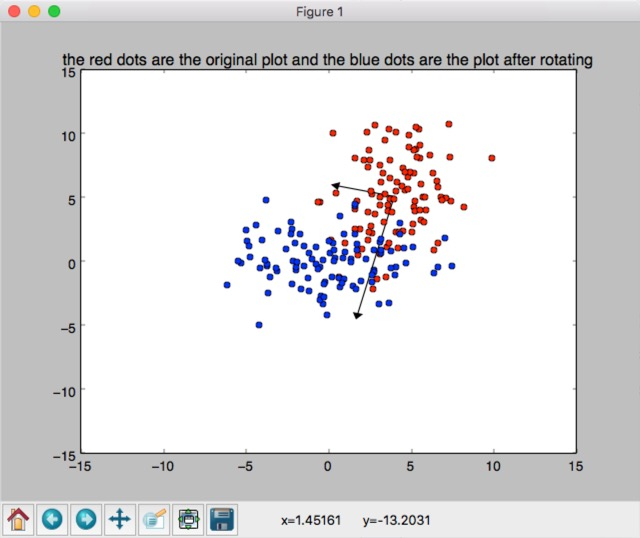
\includegraphics[scale=0.3]{q1g}
\caption{for part d and e}
\end{center}
\end{figure}
\newpage
\includepdf[pages=14]{./write.pdf}
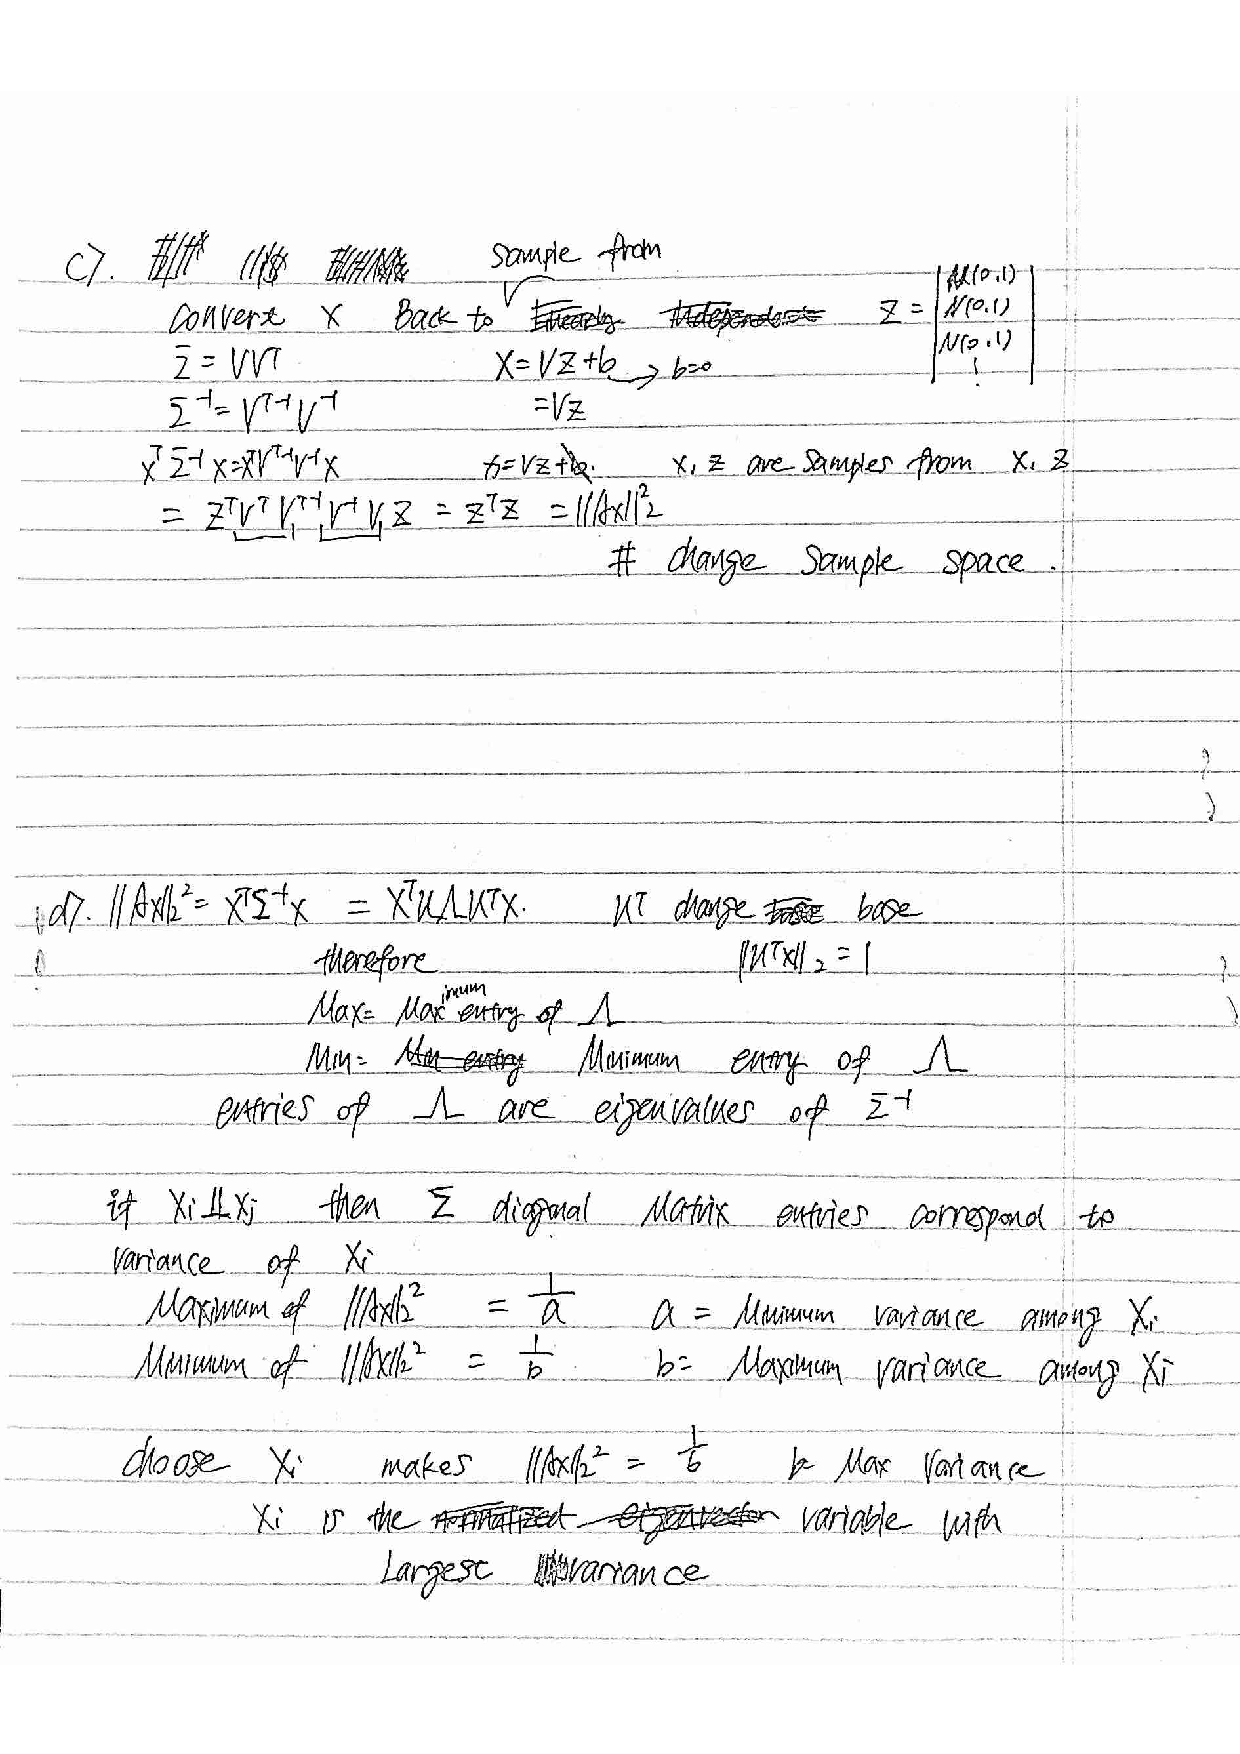
\includepdf[pages=1]{./write1.pdf}

\newpage
\section*{3.}
\begin{figure}[H]
\begin{center}
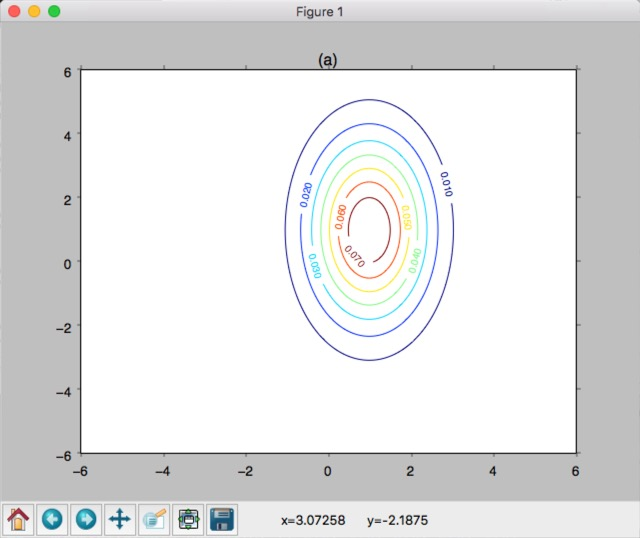
\includegraphics[scale=0.5]{3a}
\caption{a}
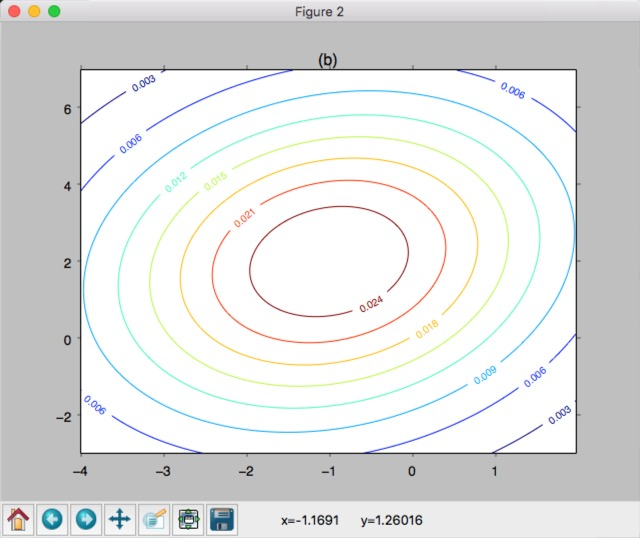
\includegraphics[scale=0.5]{3b}
\caption{b}
\end{center}
\end{figure}
\newpage
\begin{figure}[H]
\begin{center}
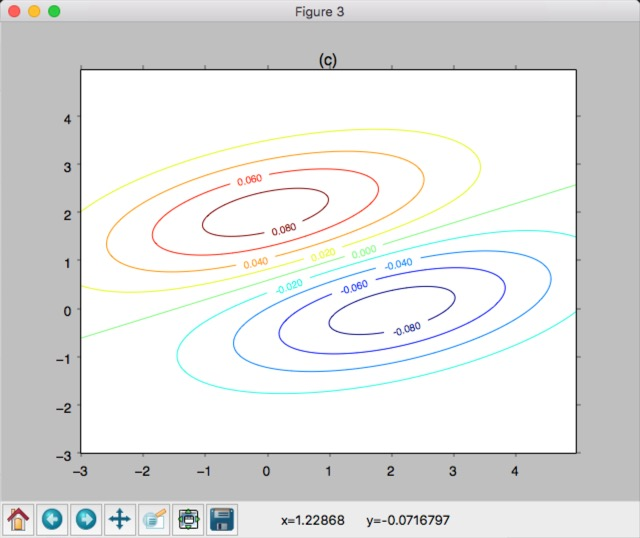
\includegraphics[scale=0.5]{3c}
\caption{c}
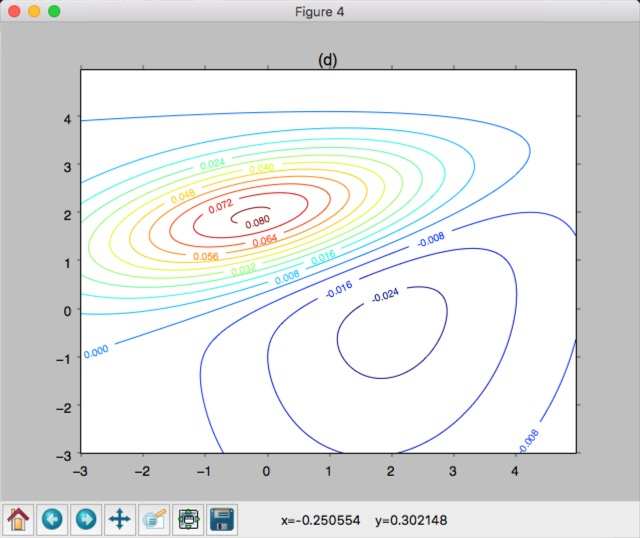
\includegraphics[scale=0.5]{3d}
\caption{d}
\end{center}
\end{figure}
\newpage
\begin{figure}[H]
\begin{center}
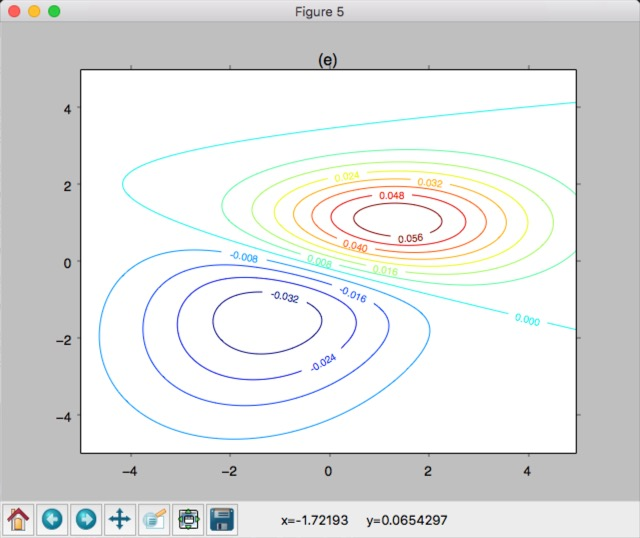
\includegraphics[scale=0.5]{3e}
\caption{e}
\end{center}
\end{figure}
\newpage
\includepdf[pages=16]{./write.pdf}
\begin{figure}[H]
\begin{center}
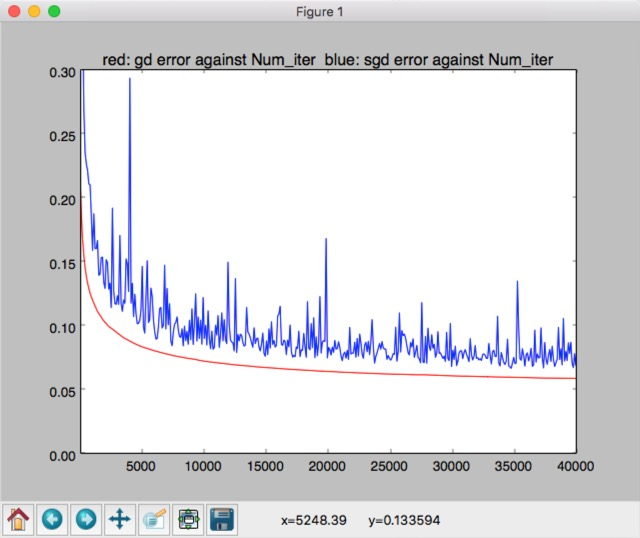
\includegraphics[scale=0.5]{reg0constant}
\caption{SGD with liear learning rate}
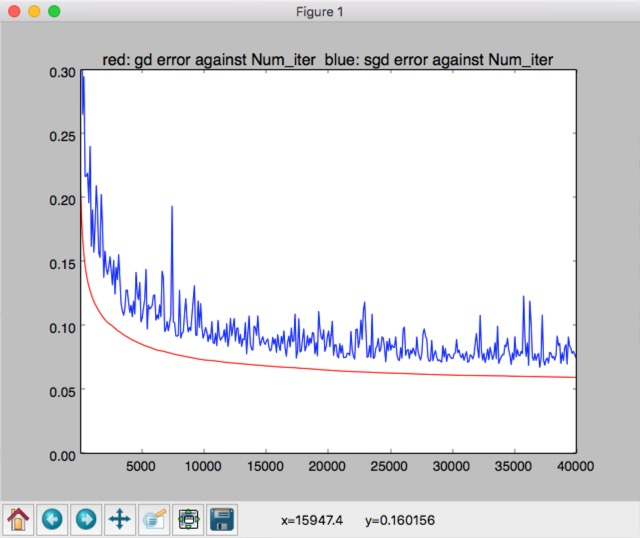
\includegraphics[scale=0.5]{reg0linear}
\caption{SGD with linear annealing learning rate}
\end{center}
\end{figure}
\section*{5}
\includepdf[pages=17]{./write.pdf}
\includepdf[pages={18-20}]{./write.pdf}
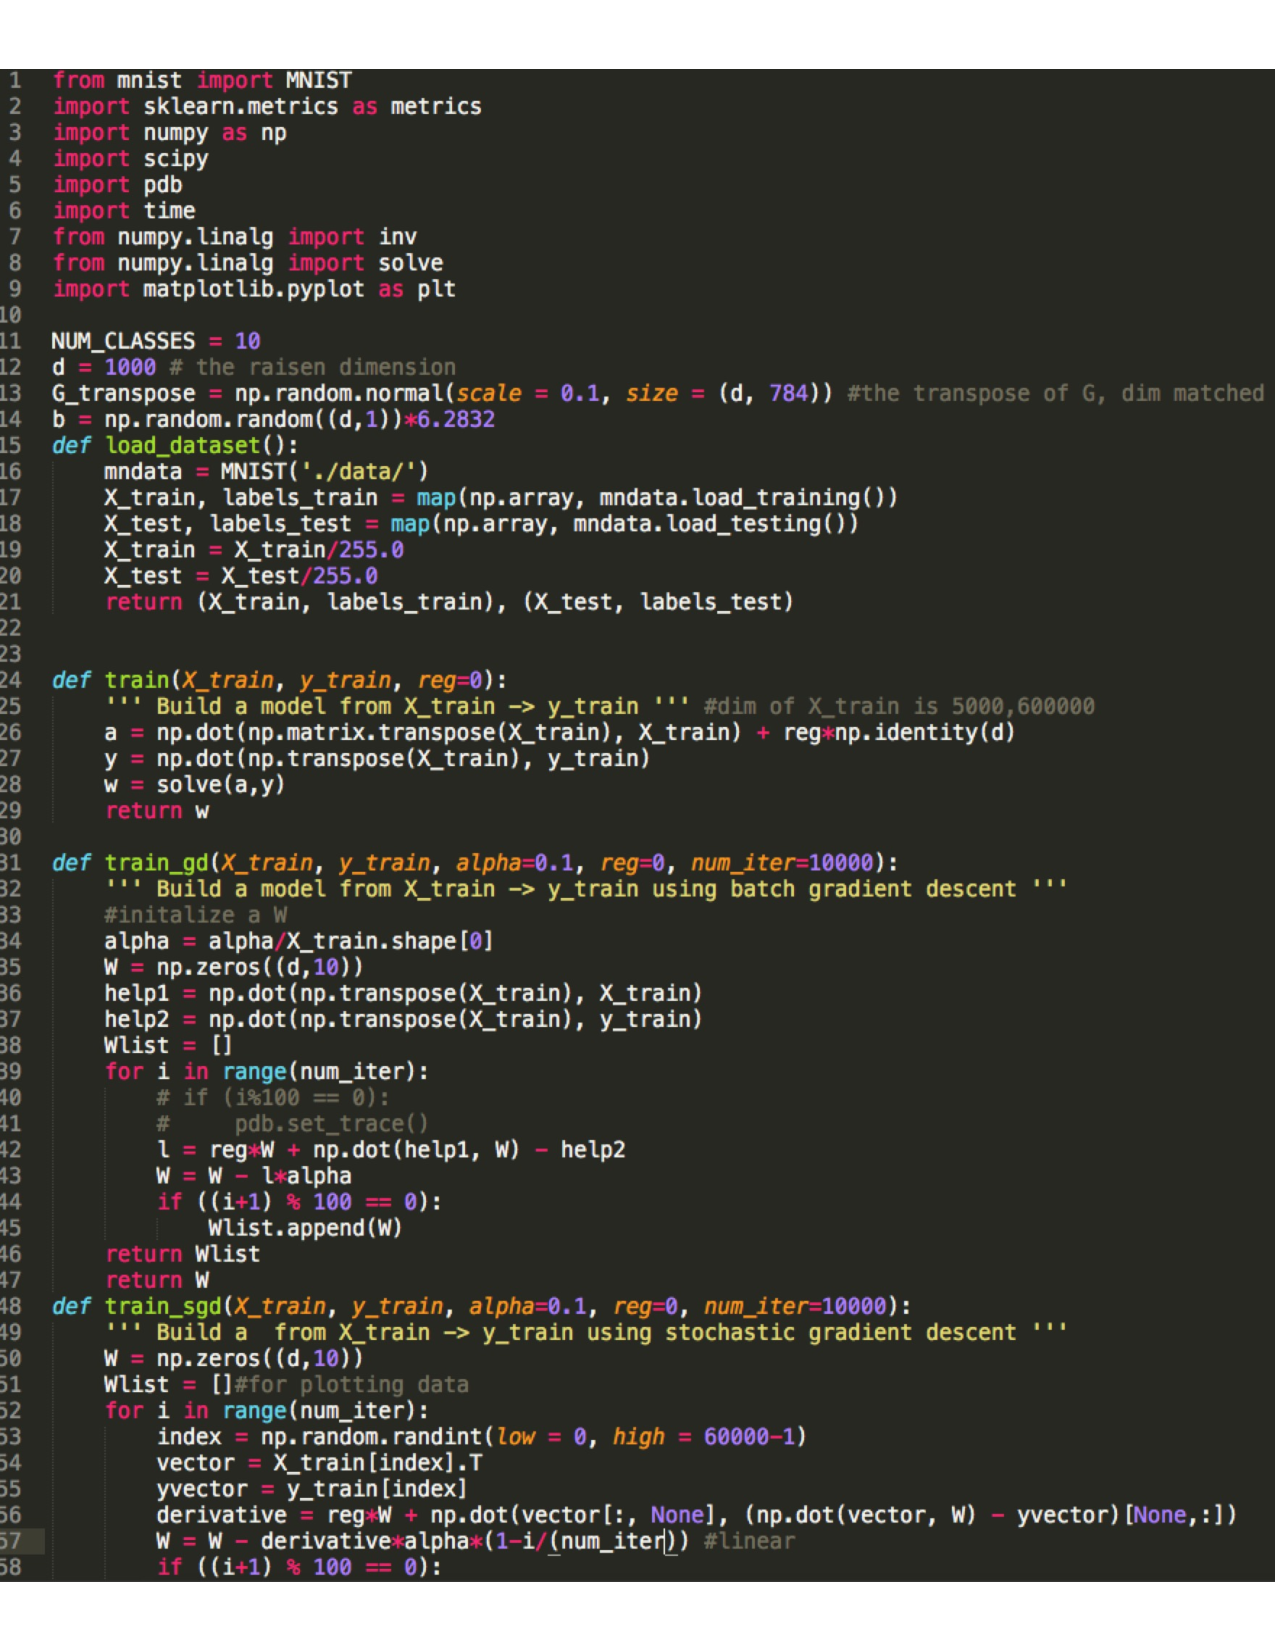
\includepdf[pages={1-3}]{./code.pdf}

\end{document}
